% !TeX root = ../../master.tex

\section{Allgemein}

Das folgende Nutzerhandbuch wurde auf die drei vorgestellten Personas angepasst, welche jeweils verschiedene Use-Cases der Anwendung darstellen sollen.
Dabei repräsentieren die Personas echte Benutzer der Anwendung.

So soll \dutzi den Dozenten darstellen, der gleichzeitig auch Administrator des Tools ist.
Dieser meldet sich dabei zunächst in der Anwendung, wie in Abschnitt~\myRefGeneral{ssec:Einloggen} beschrieben, an.
Anschließend stehen ihm verschiedene Möglichkeiten zum weiteren Vorgehen zur Verfügung.
So kann er zunächst seine eigenen veröffentlichten Umfragen einsehen und die dazugehörigen Ergebnisse betrachten, wie es in Abschnitt~\myRefGeneral{ssec:ResultDashboard} beschrieben wird.
Andererseits kann er über das \emph{Survey Master Paradise}, beschrieben in Abschnitt~\myRefGeneral{ssec:SurveyMasterParadise}, seine Umfrage-Vorlagen verwalten, neue Vorlagen erstellen und diese als konkrete Umfrage veröffentlichen.
Das Erstellen neuer Vorlagen wird in Abschnitt~\myRefGeneral{ssec:CreateMaster} näher beschrieben.

Als Administrator besitzt \dutzi ebenfalls besondere Rechte.
So ist es ihm möglich den Registrierungsschlüssel, näheres dazu in Abschnitt~\myRefGeneral{ssec:AdministratorTools}, anzuzeigen oder zu ändern.
Ebenfalls ist er imstande, einen neuen Nutzer anzulegen.
Dies ist notwendig, sofern Personen, die den Registrierungsschlüssel nicht erhalten dürfen, einen Account erhalten sollen, wie es etwa bei der Persona \ariane der Fall ist.
Zudem kann ein Administrator alle im System vorhandenen Personen einsehen, gegebenenfalls das Passwort dieser zurücksetzen oder diese zum Administrator ernennen.

Als zweite Persona wurde die Studentin \ariane vorgestellt.
Diese möchte neben der Beantwortung von Umfragen, was in Abschnitt~\myRefGeneral{ssec:TeilnahmeAnEinerUmfrage} erläutert wird, auch selbst Umfragen erstellen, was in Abschnitt~\myRefGeneral{ssec:CreateMaster} näher beschrieben wird.

Schlussendlich stellt die dritte Persona, \weigert, den typischen Studierenden dar, der lediglich an einer Umfrage teilnehmen möchte.
Dazu muss er nur die Schritte, welche in Abschnitt~\myRefGeneral{ssec:TeilnahmeAnEinerUmfrage} beschrieben werden, befolgen.
Dabei ist der benötigte Aufwand so gering wie möglich.
Der Student soll die Umfrage schnell finden und einfach beantworten können.
Zudem wird der Schutz der Daten des Teilnehmers einer solchen Umfrage besonders in den Vordergrund gerückt.
Dies liegt darin begründet, dass ein Rückschluss auf den Teilnehmer nur bei Umfragen, welche einer begrenzten Teilnehmeranzahl zur Verfügung standen, grob möglich ist.

Die meisten Funktionen, welche eine Änderung des Datenzustands zur Folge haben, besitzen zudem eine zum Anwendungsfall passende Benachrichtigung.
Einige Beispiele dazu sind in Abschnitt~\myRefGeneral{ssec:Meldungen} aufgezeigt.
Diese illustrieren alle vorhandenen Meldungstypen, die Inhalte können jedoch abweichen.

\section{Einloggen}
\label{ssec:Einloggen}

Jeder Use-Case der Anwendung beginnt mit der in Abbildung~\myRefGeneral{fig:EingabemaskeSurveycode} dargestellten Startansicht.
Um sich anzumelden, muss zunächst der mit \desTwo markierte Knopf gedrückt werden.
Hierdurch kann zur in Abbildung~\myRefGeneral{fig:Einloggen} dargestellten Seite, dem Login, gelangt werden.
Anschließend muss der Nutzer seinen vorher festgelegten Nutzernamen sowie das Passwort in die jeweiligen Felder (\desOne, \desTwo) eintragen und sich über den \emph{Login}-Knopf anmelden.
Danach erfolgt eine automatische Weiterleitung zur in Abschnitt~\myRefGeneral{ssec:ResultDashboard} abgebildeten Übersicht, der offenen Umfragen.

\begin{figure}[H]
	\centering
	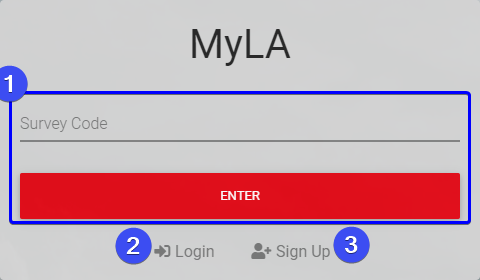
\includegraphics[width=0.5\textwidth, keepaspectratio]{img/guide/SurveyCode.png}
	\captionsetup{justification=centering, format=plain}
	\caption[Eingabemaske: Surveycodes]{Eingabemaske: Surveycodes \\\quelleScreenshot}
	\label{fig:EingabemaskeSurveycode}
\end{figure}

\begin{figure}[H]
	\centering
	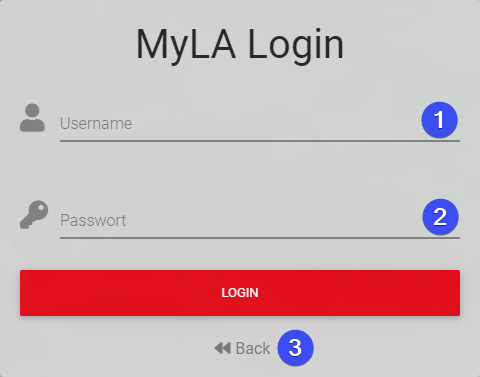
\includegraphics[width=0.5\textwidth, keepaspectratio]{img/guide/Login.png}
	\captionsetup{justification=centering, format=plain}
	\caption[Eingabemaske: Einloggen]{Eingabemaske: Einloggen \\\quelleScreenshot}
	\label{fig:Einloggen}
\end{figure}

\section{Nutzer anlegen}
\label{ssec:NutzerAnlegen}

Ein Nutzer kann über verschiedene Arten angelegt werden.
Einerseits ist es einer Person, die den Registrierungsschlüssel kennt, möglich, sich selbst zu registrieren, wie es in Abbildung~\myRefGeneral{fig:Register} gekennzeichnet wird.
Dabei muss der Nutzer in \desOne seinen gewünschten Nutzernamen, in \desTwo den festgelegten Registrierungsschlüssel und anschließend in \desThree und \desFour das gewünschte Passwort eingeben.
Falls der Registrierungsvorgang abgebrochen werden soll, kann der markierte Zurück-Knopf \desFive verwendet werden, welcher den Nutzer zurück auf die Startseite leitet.
Andererseits kann ein Administrator einen Nutzer anlegen, was jedoch genauer im Kapitel~\myRefGeneral{ssec:AdministratorTools} beschrieben wird.

\begin{figure}[H]
	\centering
	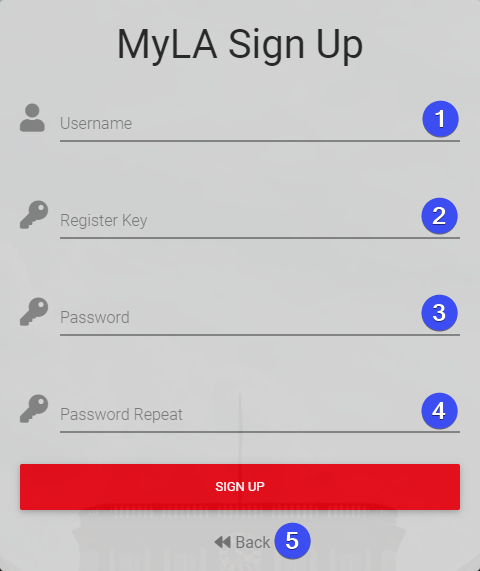
\includegraphics[width=0.5\textwidth, keepaspectratio]{img/guide/Register.png}
	\captionsetup{justification=centering, format=plain}
	\caption[Eingabemaske: Registrierung]{Eingabemaske: Registrierung \\\quelleScreenshot}
	\label{fig:Register}
\end{figure}

\section{Passwort ändern}

Jeder Nutzer ist in der Lage, sein Passwort zu ändern.
Dies kann er über sein Profil erledigen, welche über eine Funktion in der Navigationsleiste, die in Abschnitt~\myRefGeneral{ssec:NavBar} beschrieben wird, möglich ist.
Dabei muss der Nutzer zunächst, wie in Abbildung~\myRefGeneral{fig:ChangeOwnPassword} dargestellt, sein altes Passwort in \desOne angeben und in \desTwo sowie \desThree sein neues Kennwort einfügen bzw. wiederholen.
Sofern ein Nutzer sein Passwort vergisst, kann ein Administrator dieses zurücksetzen.
Dazu wählt dieser im Administrationsbereich \myRefGeneral{ssec:AdministratorTools} den jeweiligen Nutzer aus und setzt dessen Passwort über das in Abbildung~\myRefGeneral{fig:ChangePasswordOfUser} gezeigte Pop-Up neu.
Sofern der Nutzer sich mit dem neu festgelegten Passwort anmeldet, wird dieser zur eigenständigen Aktualisierung des Passworts über die vorher beschriebene Art gezwungen.

\begin{figure}[H]
	\centering
	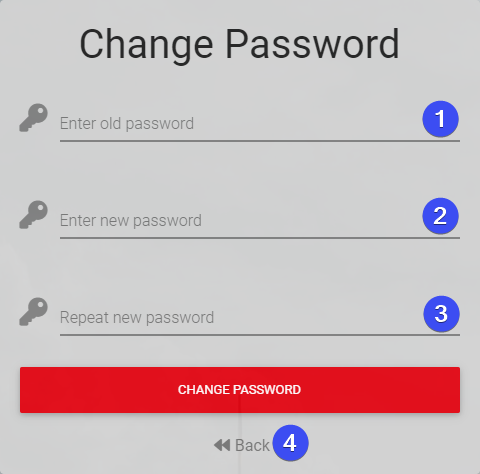
\includegraphics[width=0.5\textwidth, keepaspectratio]{img/guide/ChangeOwnPassword.png}
	\captionsetup{justification=centering, format=plain}
	\caption[Eingabemaske: Eigene Passwortänderung]{Eingabemaske: Eigene Passwortänderung \\\quelleScreenshot}
	\label{fig:ChangeOwnPassword}
\end{figure}

\begin{figure}[H]
	\centering
	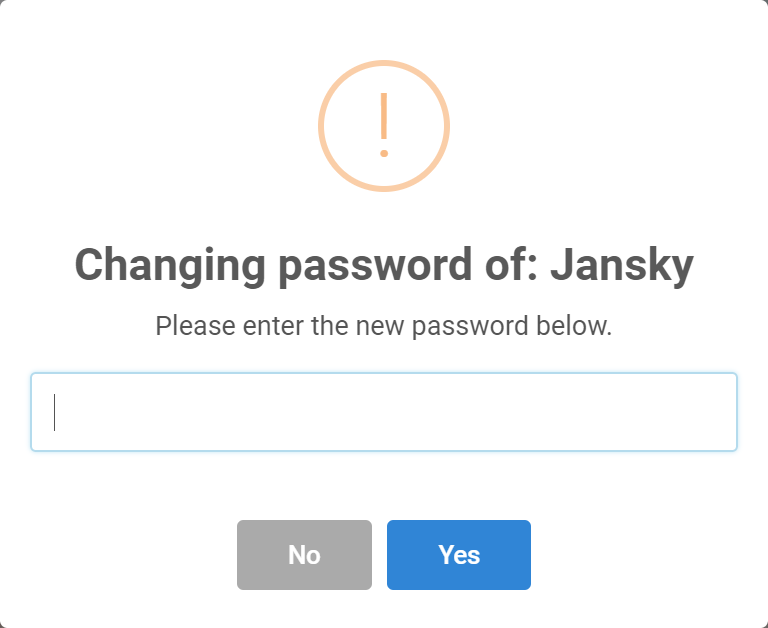
\includegraphics[width=0.5\textwidth, keepaspectratio]{img/guide/ChangePassword.png}
	\captionsetup{justification=centering, format=plain}
	\caption[Eingabemaske: Passwort zurücksetzen]{Eingabemaske: Passwort zurücksetzen \\\quelleScreenshot}
	\label{fig:ChangePasswordOfUser}
\end{figure}

\section{Result-Dashboard}
\label{ssec:ResultDashboard}

Sobald sich ein Nutzer anmeldet, wird dieser auf die Übersicht der aktiven Umfragen geleitet, dargestellt in Abbildung~\myRefGeneral{fig:ResultDashboard}.
Hier sieht der Nutzer zunächst den aktuellen Seitennamen, welcher in der Abbildung durch \desOne markiert wird.
\desTwo markiert eine Suchleiste, in der bestimmte Umfragen aus allen dargestellten Umfragen herausgefiltert werden können, sodass auch Nutzer, die bereits eine große Anzahl an Umfragen erstellt haben, ausgewählte schnell finden können.
Umfragen sind auf dieser Ansicht allgemein als Karten aufgebaut, wie \desThree zeigt.
Dabei besitzen diese einen eigenen Titel sowie den Titel der Vorlage und die Beschreibung dieser.
Zudem wird die Teilnehmeranzahl der aktiven Umfrage angezeigt, sodass der aktuelle Stand der Umfrage beobachtet werden kann, ohne die Ergebnisse explizit auswerten zu müssen.
Des Weiteren wird der Surveycode besonders hervorgehoben, um auch zu vorbereiteten Umfragen die Codes griffbereit zu haben.
\faClipboard\xspace ermöglicht es zudem den Direktlink zur Umfrage automatisch in die Zwischenablage zu kopieren, um diesen an die potenziellen Teilnehmer weiterleiten zu können.

\begin{figure}[H]
	\centering
	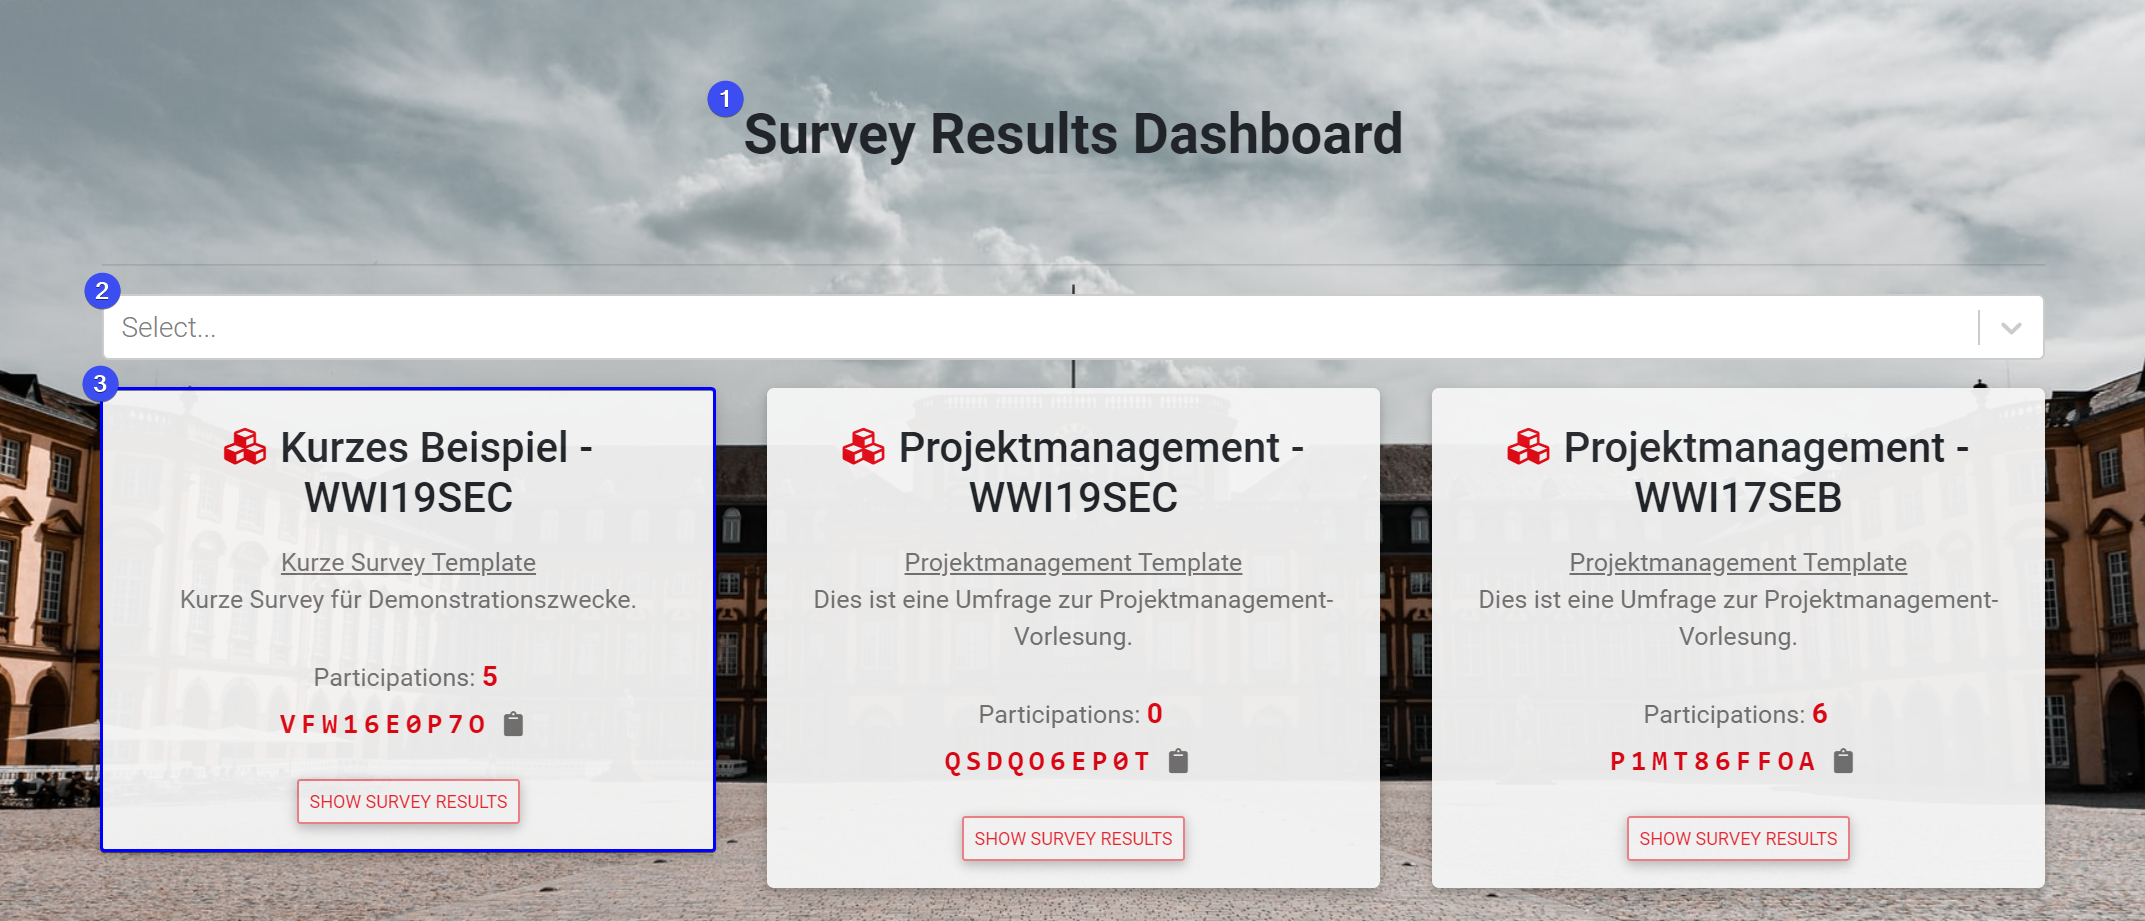
\includegraphics[width=0.95\textwidth, keepaspectratio]{img/guide/ResultDashboard.png}
	\captionsetup{justification=centering, format=plain}
	\caption[Übersicht aktiver Umfragen]{Übersicht aktiver Umfragen \\\quelleScreenshot}
	\label{fig:ResultDashboard}
\end{figure}


\section{Teilnahme an einer Umfrage}
\label{ssec:TeilnahmeAnEinerUmfrage}

Um an einer Umfrage teilzunehmen, muss der Partizipant, wie in Schritt \desOne in Abbildung~\myRefGeneral{fig:EingabemaskeSurveycode} dargestellt, einen \emph{Surveycode} eingeben.
Da das Teilnehmen an Umfragen einen Kernpunkt der Anwendung darstellt, ist dies das zentrale Element der Startseite.

\begin{figure}[H]
	\centering
	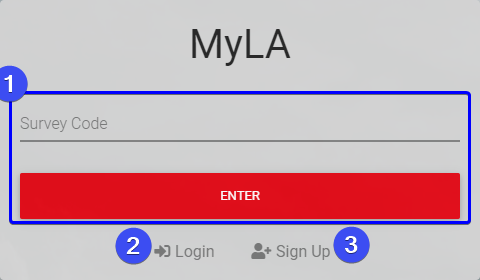
\includegraphics[width=0.5\textwidth, keepaspectratio]{img/guide/SurveyCode.png}
	\captionsetup{justification=centering, format=plain}
	\caption[Eingabemaske: Surveycode]{Eingabemaske: Surveycode \\\quelleScreenshot}
	\label{fig:EingabemaskeSurveycode}
\end{figure}

Abbildung~\myRefGeneral{fig:Teilnehmermaske} stellt die Teilnehmermaske der Umfrage dar.
\desOne zeigt den Titel der Umfrage (hier: Projektmanagement -- WWI17SEB).
\desTwo zeigt die Beschreibung der Umfrage (hier: Dies ist eine Umfrage zur Projektmanagement-Vorlesung).
\desThree ist das Hauptelement der Seite, was die Umfrage darstellt.
Über den Knopf \enquote{Complete} kann der Teilnehmer die Umfrage abschließen.
Er erhält im Anschluss ein visuelles Feedback.
%
\begin{figure}[H]
	\centering
	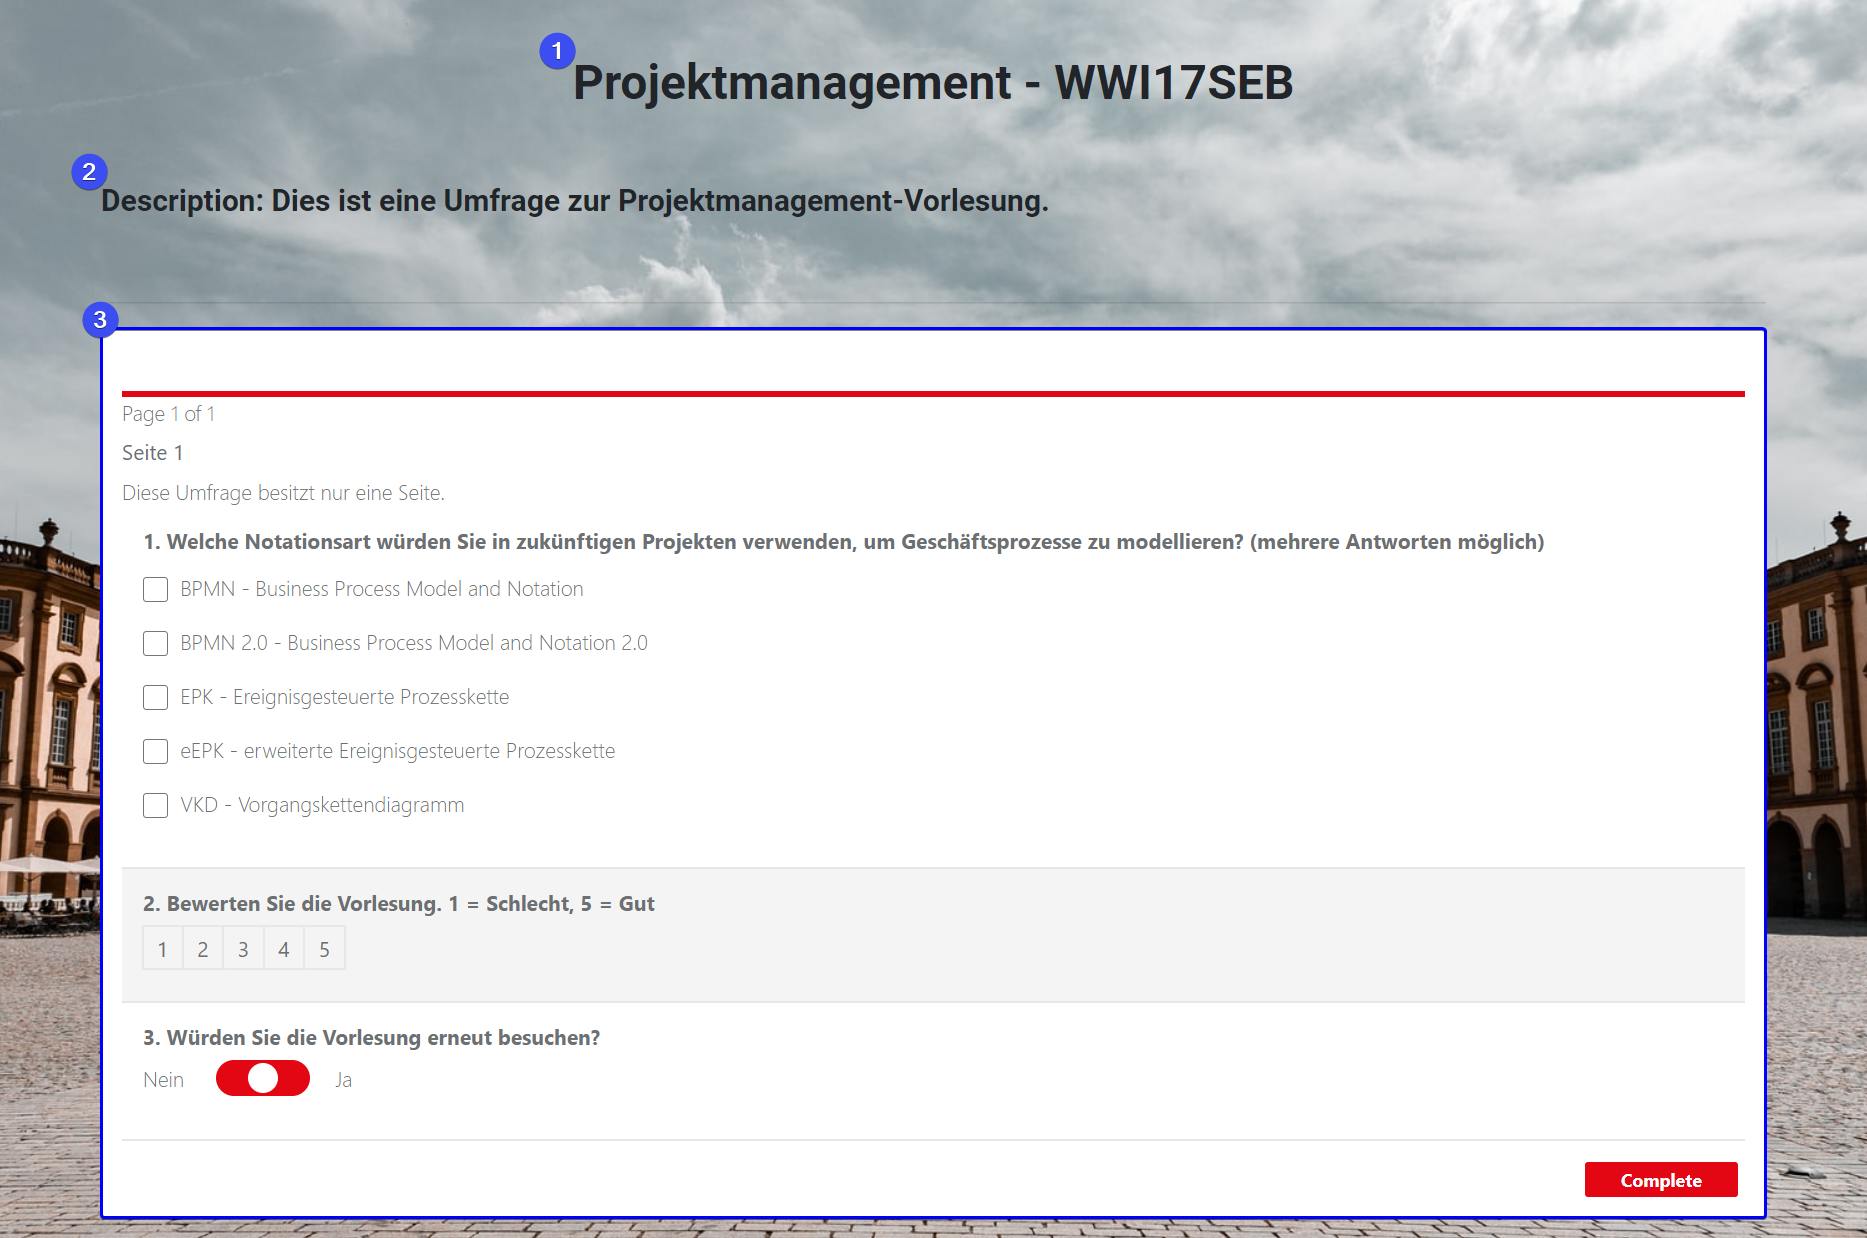
\includegraphics[width=0.95\textwidth, keepaspectratio]{img/guide/SurveyParticipate.png}
	\captionsetup{justification=centering, format=plain}
	\caption[Eingabemaske: Benutzerumfrage]{Eingabemaske: Benutzerumfrage \\\quelleScreenshot}
	\label{fig:Teilnehmermaske}
\end{figure}
%
\section{Erstellen einer Umfrage}
\label{ssec:CreateMaster}

Das Kernelement dieser Anwendung ist das Erstellen von Umfragen.
Abbildung~\myRefGeneral{fig:Umfrageeditor} zeigt den Editor zum Erstellen oder Bearbeiten einer Umfrage. \newline
Der Benutzer kann hier einen Titel und eine Beschreibung für seine Umfrage wählen.
Über den in der linken Seite befindlichen Navigationsbereich kann der Benutzer verschiedene Elemente wie \ua:
%
\begin{itemize}
    \item Single-/Multiple Choice,
    \item Ja/Nein Antworten,
    \item Freitextfeld (Single-Input),
    \item Bewertungsskala (Skala frei wählbar),
    \item Auswahl von Bildern
\end{itemize}
%
verwenden.

Im oberen Bereich des Editors befindet sich die Seitenverwaltung.
Der Benutzer kann hier seine Umfrage strukturieren, indem er der Umfrage eine neue Seite hinzufügt.
Darüber hinaus kann er stets zwischen den Seiten wechseln.

Der im rechten Teil befindliche Navigationsbereich beinhaltet \ua die Menüsprache (hier: Englisch).
Darüber hinaus können Beantwortungszeiten festgelegt werden, die die maximale Dauer zum Ausfüllen der Umfrage definieren.

Über den Knopf \enquote{Save Survey} kann der Benutzer seine Umfrage speichern.
Er erhält ein entsprechendes visuelles Feedback.

\begin{figure}[H]
	\centering
	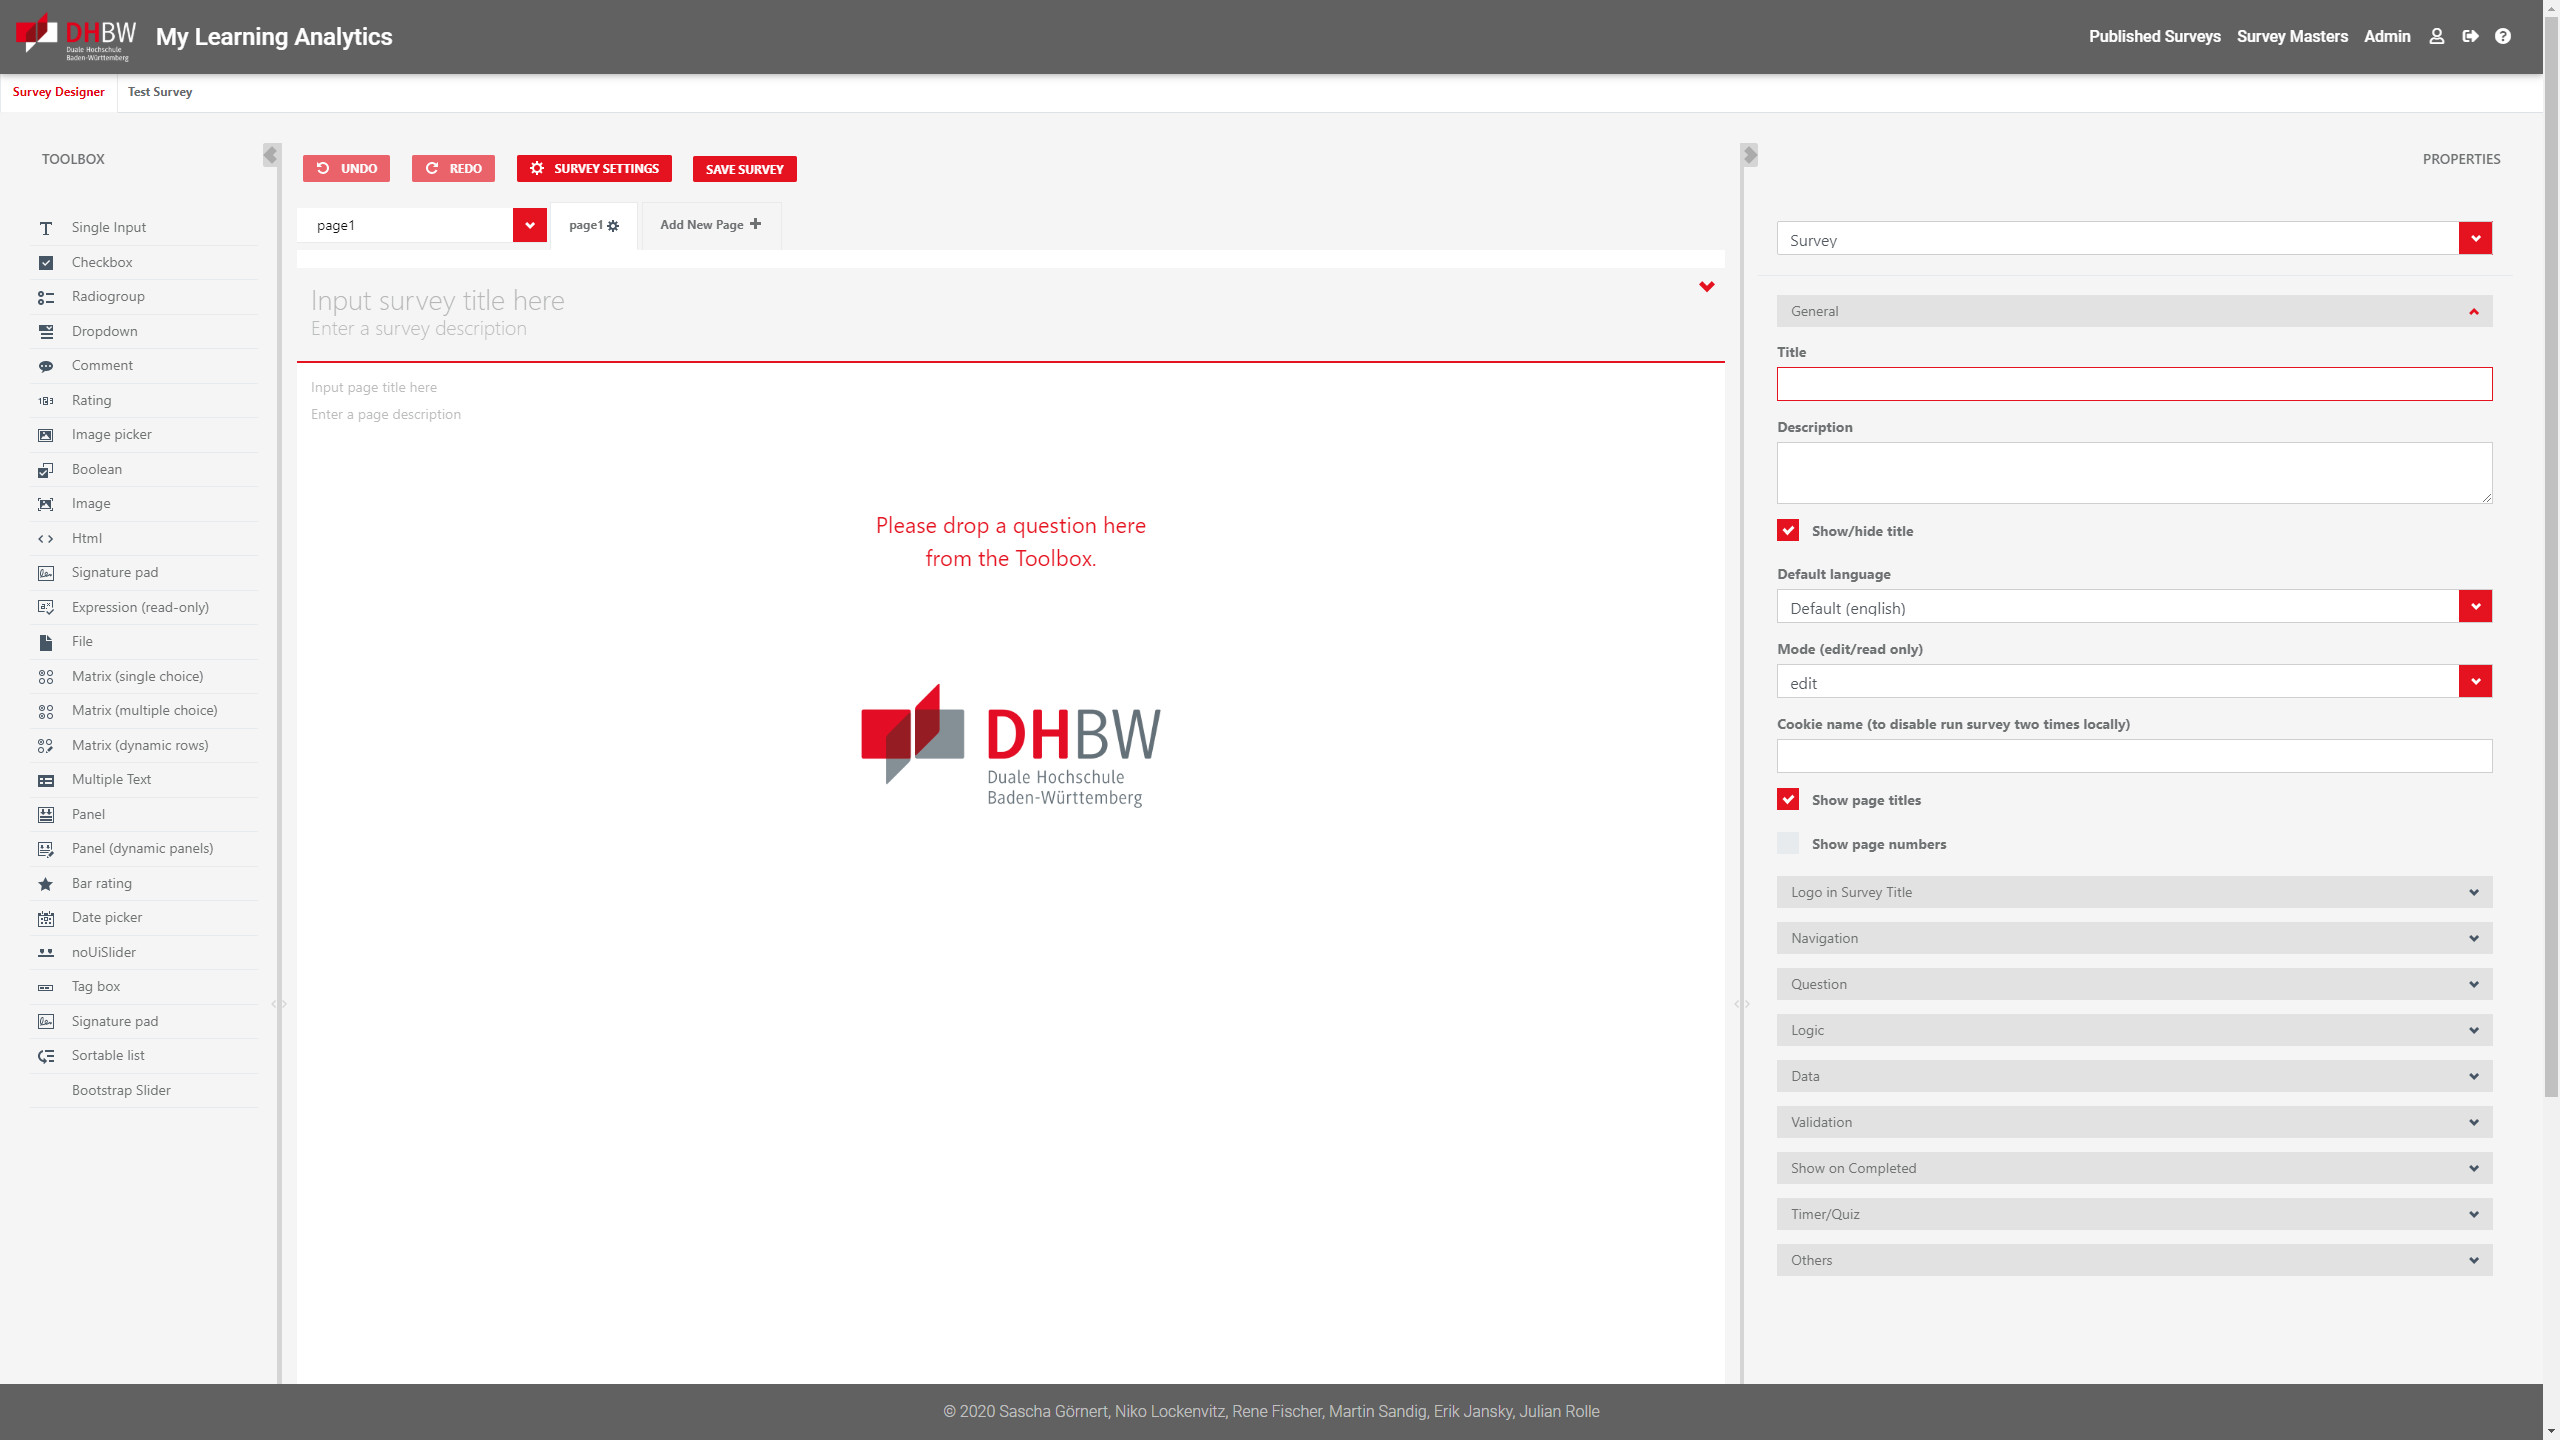
\includegraphics[width=0.95\textwidth, keepaspectratio]{img/guide/SurveyTemplate.png}
	\captionsetup{justification=centering, format=plain}
	\caption[\acl{UI}: Umfrageeditor]{\acl{UI}: Umfrageeditor \\\quelleScreenshot}
	\label{fig:Umfrageeditor}
\end{figure}

\section{Administrator-Tools}
\label{ssec:AdministratorTools}

Abbildung~\vref{fig:AdminSpace} zeigt den Administrationsbereich der Anwendung.
Der Benutzer kann hier, wie durch \desOne markiert, den Registrierungsschlüssel zum Registrieren eines neuen Benutzers einsehen oder neu festlegen (vgl. Abbildung~\vref{fig:EditRegisterKey} sowie Abbildung~\vref{fig:NewRegisterkey}). \newline
\desTwo zeigt die Möglichkeit des Erstellens eines neuen Benutzers (vgl. Abbildung~\vref{fig:NeuenBenutzerAnlegen}).
Über die mit \desThree hervorgehobene Karte kann der Administrator alle Benutzer im System anzeigen lassen (vgl. Abbildung~\vref{fig:UserSpace}).

\begin{figure}[H]
	\centering
	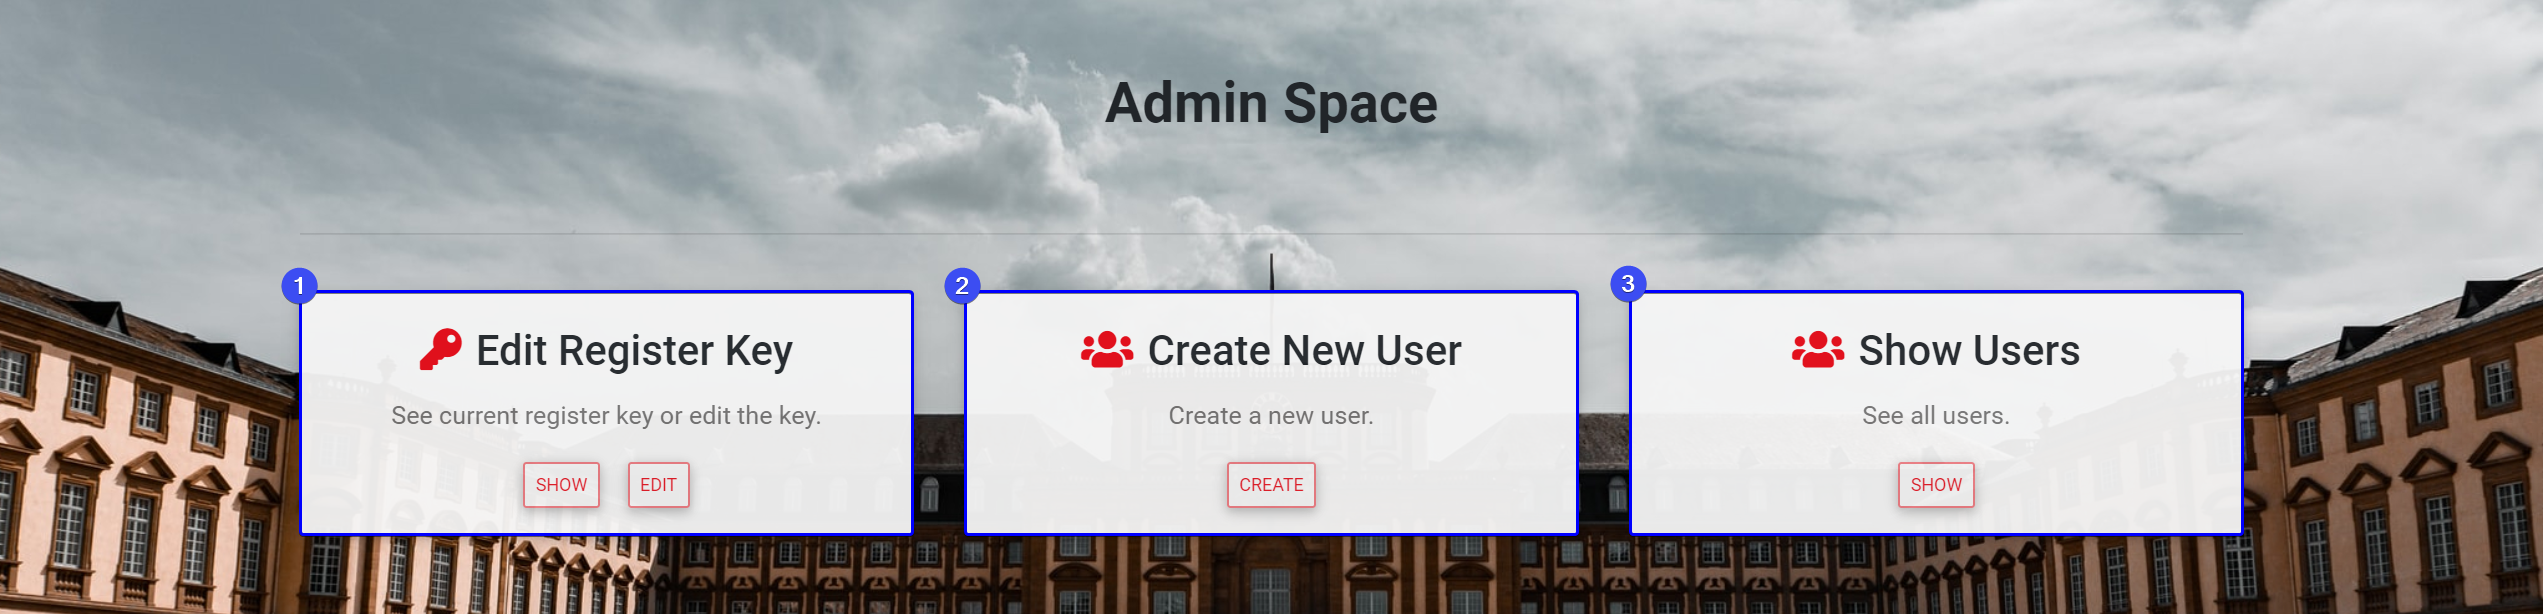
\includegraphics[width=0.95\textwidth, keepaspectratio]{img/guide/AdminSpace.png}
	\captionsetup{justification=centering, format=plain}
	\caption[\acl{UI}: Administrationsbereich]{\acl{UI}: Administrationsbereich \\\quelleScreenshot}
	\label{fig:AdminSpace}
\end{figure}

\begin{figure}[H]
	\centering

	
\includegraphics[width=0.5\textwidth, keepaspectratio, trim=2mm 0 2mm 0, clip]{img/guide/RegisterKey.png}
	\captionsetup{justification=centering, format=plain}
	\caption[Meldung: Neuer Registrierungsschlüssel]{Meldung: Neuer Registrierungsschlüssel \\\quelleScreenshot}
	\label{fig:NewRegisterkey}
\end{figure}

\begin{figure}[H]
	\centering
	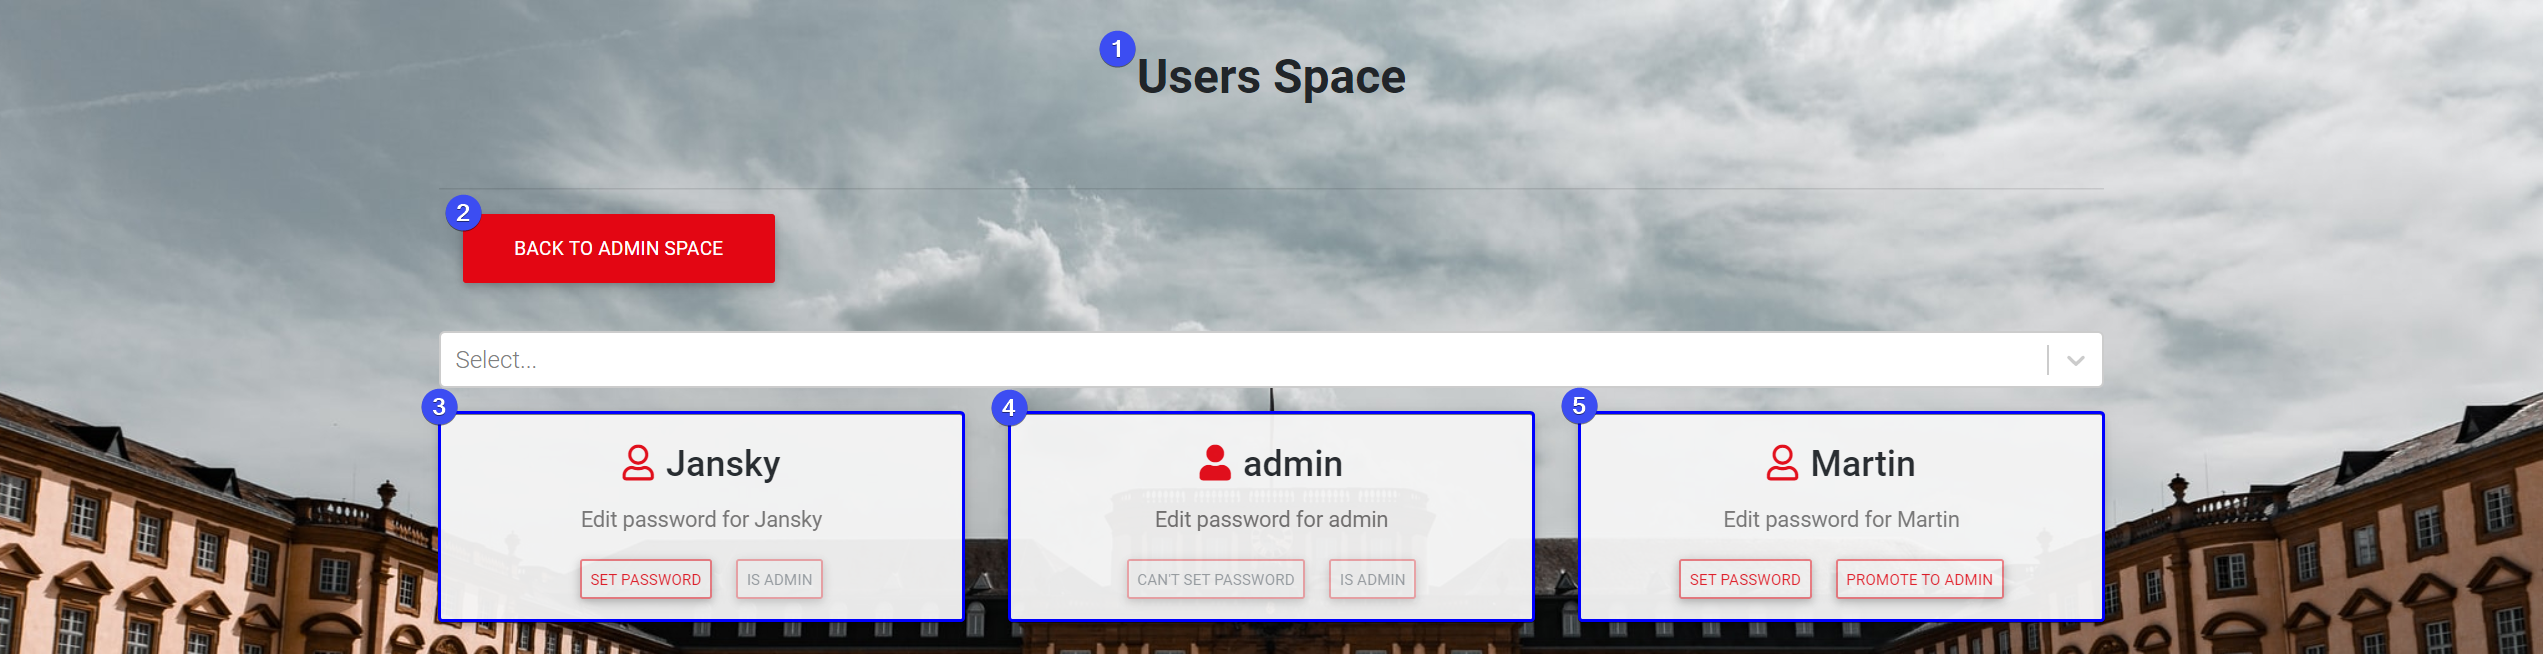
\includegraphics[width=0.95\textwidth, keepaspectratio]{img/guide/UserSpace.png}
	\captionsetup{justification=centering, format=plain}
	\caption[\acl{UI}: Auflistung der Nutzer]{\acl{UI}: Auflistung der Nutzer \\\quelleScreenshot}
	\label{fig:UserSpace}
\end{figure}

\begin{figure}[H]
	\centering
	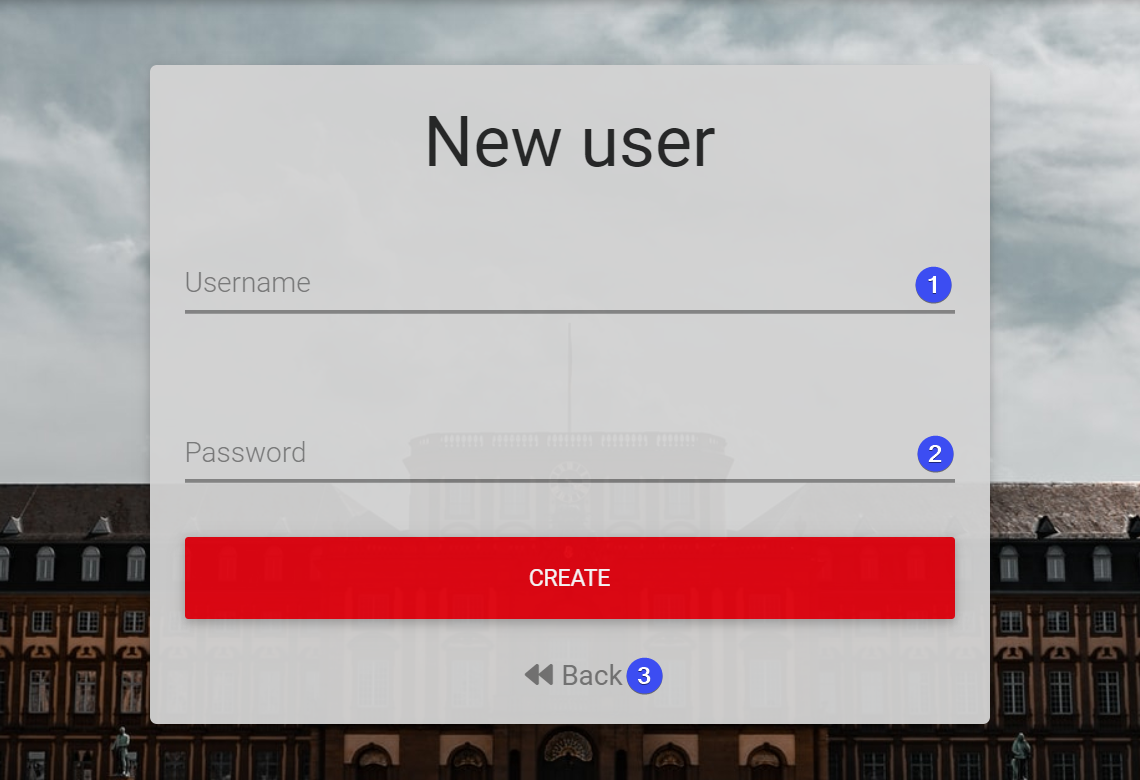
\includegraphics[width=0.50\textwidth, keepaspectratio]{img/guide/NewUser.png}
	\captionsetup{justification=centering, format=plain}
	\caption[Eingabemaske: Neuen Benutzer anlegen]{Eingabemaske: Neuen Benutzer anlegen \\\quelleScreenshot}
	\label{fig:NeuenBenutzerAnlegen}
\end{figure}

\begin{figure}[H]
	\centering
	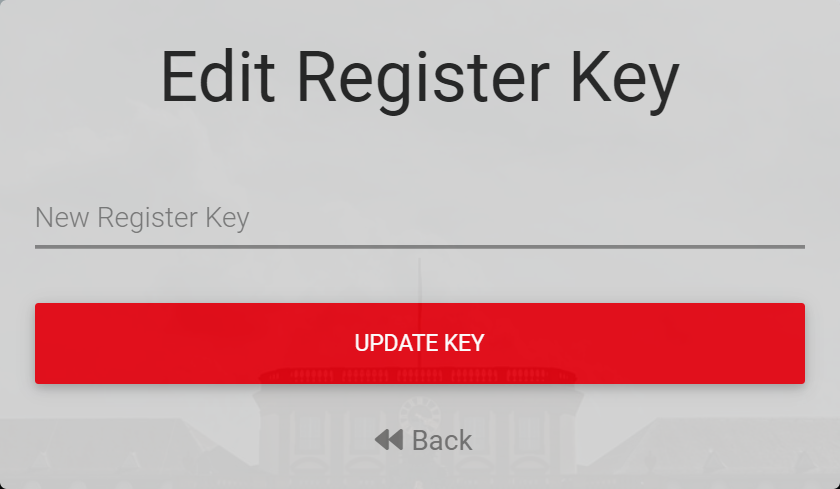
\includegraphics[width=0.5\textwidth, keepaspectratio]{img/guide/EditRegisterKey.png}
	\captionsetup{justification=centering, format=plain}
	\caption[Eingabemaske: Editieren des Registrierungsschlüssels]{Eingabemaske: Editieren des Registrierungsschlüssels \\\quelleScreenshot}
	\label{fig:EditRegisterKey}
\end{figure}



%%%%%%%%% --------------------- %%%%%%%%%%%%%%%
\section{My Account}
\label{ssec:EigenerAccount}

Zur Verwaltung des Benutzerkontos von etwa \dutzi oder \ariane, kann die in Abbildung~\myRefGeneral{fig:MyAccount} dargestellte Benutzeroberfläche verwendet werden.
In der Oberfläche können Nutzer \ua ihr Passwort ändern.
Abbildung~\myRefGeneral{fig:ChangeOwnPassword} zeigt die Passwortwechsel-Oberfläche.
Um das Ändern des Passworts zu bestätigen, müssen diese in \desOne zuerst ihr altes Passwort eingeben.
Anschließend muss in \desTwo das neue Passwort eingegeben und in \desThree bestätigt werden.
Über den Knopf \enquote{Change Password} wird die Aktion dann ausgeführt.
Alternativ kann über den Zurück-Knopf \desFour wieder auf die Benutzeroberfläche navigiert werden.
%
\begin{figure}[H]
	\centering
	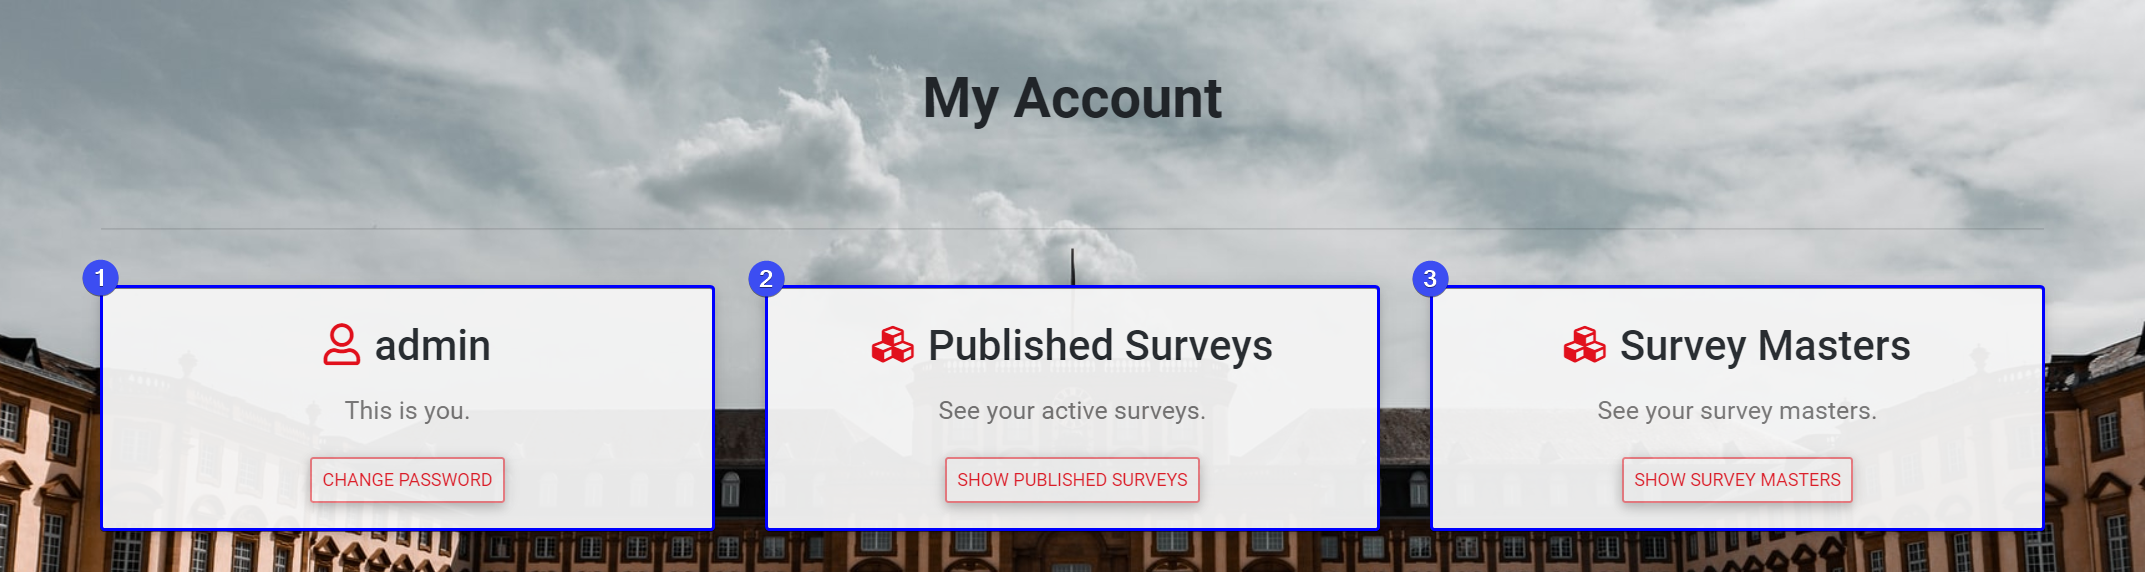
\includegraphics[width=0.95\textwidth, keepaspectratio]{img/guide/MyAccount.png}
	\captionsetup{justification=centering, format=plain}
	\caption[\acl{UI}: My Account]{\acl{UI}: My Account\\\quelleScreenshot}
	\label{fig:MyAccount}
\end{figure}
%
\begin{figure}[H]
	\centering
	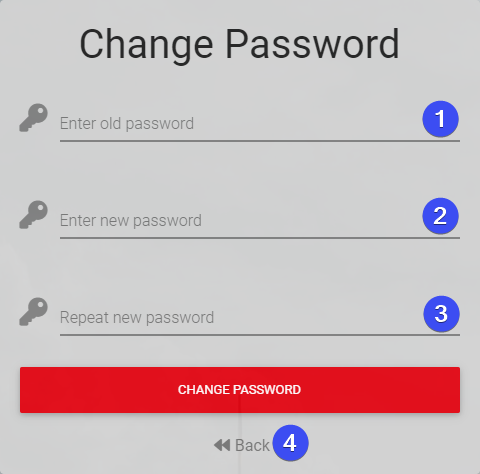
\includegraphics[width=0.5\textwidth, keepaspectratio]{img/guide/ChangeOwnPassword.png}
	\captionsetup{justification=centering, format=plain}
	\caption[Eingabemaske: Passwortänderung (Benutzeransicht)]{Passwortänderung (Benutzeransicht)\\\quelleScreenshot}
	\label{fig:ChangeOwnPassword}
\end{figure}
%
%%%%%%%%% --------------------- %%%%%%%%%%%%%%%
\section{Survey Master Paradise}
\label{ssec:SurveyMasterParadise}
Survey Master Paradise ist eine der Hauptkomponenten dieser Anwendung.
Hier können die Benutzer der Anwendung, wie \dutzi oder \ariane, ihre erstellen Umfragen einsehen.
Abbildung~\vref{fig:SurveyMasterParadise} zeigt die Umfrageseite. \newline
Die Ansicht dient dazu, eine Übersicht zu angelegten Umfragen zu geben.
Zudem können Umfragen veröffentlicht werden, welche zuvor benannt werden müssen.
Aufgrund der Vielzahl an Umfragen, die nach einer gewissen Nutzungszeit entstanden sind, wurde die Suchfunktion \desTwo eingefügt, welche Vorlagen nach dem Umfragenamen wie \zb \emph{Projektmanagement Template} filtert.
Über \desThree können die Benutzer eine neue Vorlage erstellen (vgl. Abschnitt~\vref{ssec:CreateMaster}). \newline
Mit Hilfe von \desFour werden Vorlagen unter einem bestimmten Titel publiziert (Publish Survey).
Die Anzahl der Publikationen ist für die Nutzer ersichtlich (Times published). \newline
Die Icons, wie in \desFive dargestellt, bieten dem Benutzer die Möglichkeit, sofern er noch keine Umfrage publiziert hat:
%
\begin{itemize}
    \item seine Umfrage zu editieren \faEdit
    \item seine Umfrage zu kopieren \faCopy
    \item oder zu löschen \faTrash.
\end{itemize}
%
Hat \zb \dutzi mindestens eine Umfrage, basierend auf seiner Vorlage, publiziert, so stehen ihm noch die Funktionen:
%
\begin{itemize}
    \item Umfrage kopieren \faCopy
    \item und \faIdCard
\end{itemize}
%
zur Verfügung.
%
\begin{figure}[H]
	\centering
	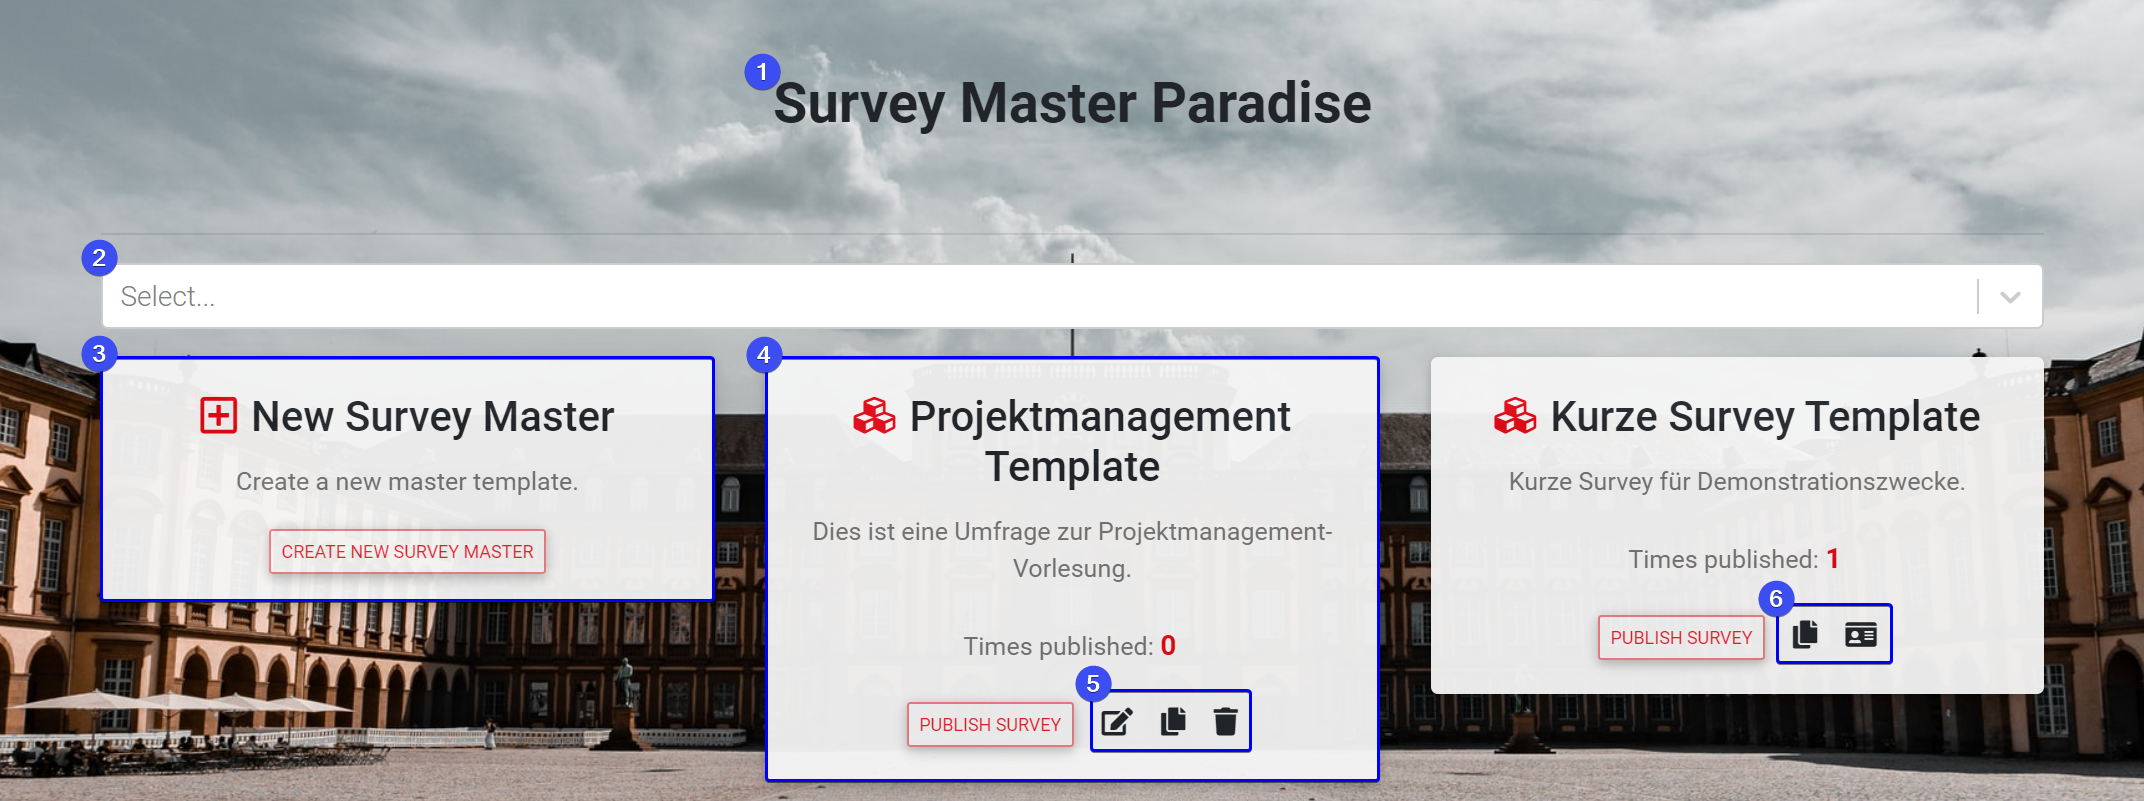
\includegraphics[width=0.95\textwidth, keepaspectratio]{img/guide/SurveyMasterParadise.png}
	\captionsetup{justification=centering, format=plain}
	\caption[\acl{UI}: Survey Master Paradise]{\acl{UI}: Survey Master Paradise \\\quelleScreenshot}
	\label{fig:SurveyMasterParadise}
\end{figure}
%
%%%%%%%%% --------------------- %%%%%%%%%%%%%%%
\section{Navigationsbereich}
\label{ssec:NavBar}

In Abbildung~\vref{fig:NavBar} ist ein Ausschnitt der oberen Navigationsleiste sichtbar.
Die Benutzer können über \desOne zu ihren Umfrageergebnissen navigieren (vgl. Abschnitt~\vref{ssec:ResultDashboard}).
\ariane könnte hier zum Beispiel die Ergebnisse ihrer Bachelorarbeit validieren.
Der mit \desTwo markierte Link führt auf die Umfragevorlagen (vgl. Abschnitt~\vref{ssec:SurveyMasterParadise}).
Hier kann \dutzi \zb eine weitere Vorlage anlegen und für seinen neuen Kurs \emph{WWWI20MAC} publizieren.

Ferner zeigt die Navigationsleiste den Status \emph{Admin} \desThree, im Falle, dass der Benutzer ein administrative Rolle hat. \newline
Über das Icon \faUser[regular]\xspace \desFour kann der Benutzer zu seinem Account navigieren (vgl. Abschnitt~\vref{ssec:EigenerAccount}). \newline
Über \desFive das Logout-Icon \faSignOut*\xspace können sich \dutzi oder die Studentin \ariane vom System abmelden.

\begin{figure}[H]
	\centering
	
\includegraphics[width=0.75\textwidth, keepaspectratio]{img/guide/NavBar.png}
	\captionsetup{justification=centering, format=plain}
	\caption[Navigationsbereich]{Navigationsbereich \\\quelleScreenshot}
	\label{fig:NavBar}
\end{figure}

%%%%%%%%% --------------------- %%%%%%%%%%%%%%%
\section{Meldungen}
\label{ssec:Meldungen}

Nachfolgend sind alle Meldungsarten mit Beispielen dargestellt.
Zunächst wird in Abbildung~\myRefGeneral{fig:approve} eine kurzzeitig eingeblendete Bestätigung dargestellt, welche eine Nachricht, die an den aktuellen Kontext angepasst ist, beinhaltet.
Bestätigungen werden in den meisten Fällen automatisch ein- und ausgeblendet, um den Benutzerfluss nicht zu stören.
Im Beispiel wird dem Administrator bestätigt, dass er einen weiteren Nutzer zum Administrator ernannt hat.

Auch abgelehnte oder abgebrochene Auftrage werden mit einer Nachricht versehen.
Diese beinhalten jedoch immer einen Knopf zur Bestätigung, sodass Fehlermeldungen auch wahrgenommen oder weiteren Personen gezeigt werden können.
Ein Beispiel hierfür wird in Abbildung~\myRefGeneral{fig:deny} gezeigt.
Bei diesem wird die Passwortänderung des Nutzers \emph{Jansky} abgebrochen.

Auch Warnungen erhalten eine besondere Darstellung.
Hierbei werden Änderungen, die eine Nutzereingabe benötigen, oder generelle Infos, die weder als negative noch als positive Benachrichtigung zu zählen sind, dargestellt.
Dazu wird ebenfalls eine Bestätigung durch ein \emph{OK} oder eine explizite Auswahl, repräsentiert durch zwei Knöpfe, welche kontextsensitiv sind, zur Bestätigung verwendet.
In der nachfolgenden Abbildung~\ref{fig:warn} wird ein Beispiel gezeigt, bei dem eine Umfrage veröffentlicht wird, welche einen eigenen Titel benötigt und somit ein Eingabefeld beinhaltet.

Zu guter Letzt gibt es weitere Sonderbenachrichtigungen, die wiederum kontextabhängig sind.
So ist in der nachfolgenden Abbildung~\ref{fig:special} die Bestätigung einer veröffentlichten Umfrage, welche nicht automatisch ausgeblendet wird, sondern aufgrund des besonderen Inhalts länger dargestellt wird und vom Nutzer selbst ausgeblendet werden muss, dargestellt.
Hierbei werden ebenfalls besondere Bestandteile visuell hervorgehoben, wie etwa der Surveycode in der Beispiel-Abbildung.

\begin{figure}[H]
	\centering
	
\includegraphics[width=0.5\textwidth, keepaspectratio]{img/guide/Angenommen.png}
	\captionsetup{justification=centering, format=plain}
	\caption[Meldung: Bestätigung]{Beispiel: Bestätigung \\\quelleScreenshot}
	\label{fig:approve}
\end{figure}

\begin{figure}[H]
	\centering
	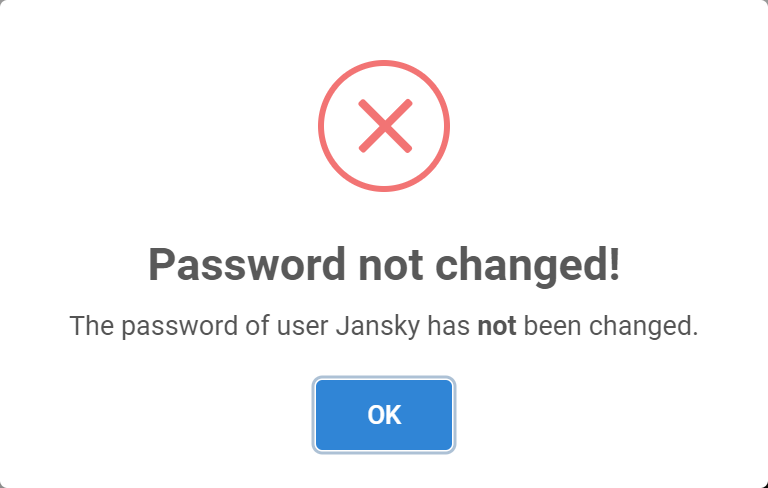
\includegraphics[width=0.5\textwidth, keepaspectratio]{img/guide/Abgelehnt.png}
	\captionsetup{justification=centering, format=plain}
	\caption[Meldung: Ablehnung]{Beispiel: Ablehnung \\\quelleScreenshot}
	\label{fig:deny}
\end{figure}

\begin{figure}[H]
	\centering
	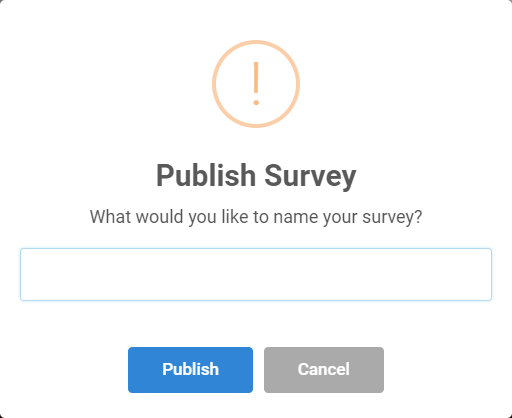
\includegraphics[width=0.5\textwidth, keepaspectratio]{img/guide/Publish.png}
	\captionsetup{justification=centering, format=plain}
	\caption[Meldung: Warnung mit Input]{Beispiel: Warnung mit Input \\\quelleScreenshot}
	\label{fig:warn}
\end{figure}

\begin{figure}[H]
	\centering
	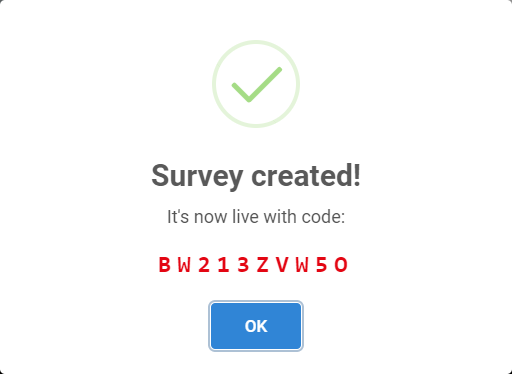
\includegraphics[width=0.5\textwidth, keepaspectratio]{img/guide/Published.png}
	\captionsetup{justification=centering, format=plain}
	\caption[Meldung: Bestätigung mit Zusatz]{Beispiel: Bestätigung mit Zusatz \\\quelleScreenshot}
	\label{fig:special}
\end{figure}
